\documentclass[]{report}

\usepackage{amsmath,amsfonts}
\usepackage{graphicx}
\usepackage{url}
\usepackage[hidelinks]{hyperref}

% Title Page
\title{{\huge  TITLE} \\
{\small Automatic Control\\
Electronic Engineering for Intelligent Vehicles\\
University of Bologna\\
A.A. 202X-202X}}
\author{Student A and Student B and ...}


\begin{document}
\maketitle

\begin{abstract}
	Here briefly detail  the aims of the project.
\end{abstract}

\chapter{Introduction}
\section{Motivations}
Explain why the selected application is important. Describe the application with informal words.

\section{Contributions}
Describe what this project deals with. What has been done to solve the problem presented in the motivations.

\section{State of art and literature comparison}
List the closest works that deal with the same problem and compare the achievement obtained and the strategies exploited in this paper. For the search of the literature use \url{https://ieeexplore.ieee.org/Xplore/home.jsp} and \url{https://www.sciencedirect.com/}.

\section{Organisation of the manuscript}
Describe what the reader finds in each of the Sections of this manuscript.

\section{List of the symbols}
Here list all the symbols used in the manuscript and add a description to each of them (Use the International System of Units \url{https://en.wikipedia.org/wiki/International_System_of_Units}).

\chapter{MAIN BODY}
Change the title with the name of the selected application

\section{Model and Problem Formulation}
Here describe the  model and state the problem with a mathematical formalism.

To add formulas use the environment \textit{equation} and add a label to which the reader can refer. As example
\begin{equation}
	\label{eq:FormulaA}
	\begin{aligned}
		\dot{x} &= f(x,u) && x(t_0) = x_0
\\
y &= h(x,u)
\end{aligned}
\end{equation}
To insert a hyperlink to the formula use the environment \textit{eqref}. As example \eqref{eq:FormulaA}.

\section{Model Analysis}
Analyse the plant: Linearisation, Eigenvalues, Observability, Reachability.

\section{Proposed Solution}
Here describe the proposed solution: Control system architecture (draw a block scheme!), mathematical description of the solution, listings of the MATLAB code implemented to obtain the solution

To include a picture use the environment \textit{figure}. 
\begin{figure}[h!]
	\centering
	%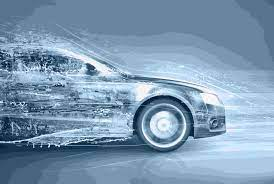
\includegraphics[width=0.7\columnwidth]{Figure}
	\caption{Add the caption to each figure! The caption should completely describe the figure so that the reader should be able to understand it without the need of reading the main text.}
	\label{fig:FigureA}
\end{figure}
Use the environment \textit{ref} to add a hyperlink to the figure. As example Figure \ref{fig:FigureA}.

\chapter{Application}

\section{Simulator description}
Copy and past the Simulink block scheme and describe what each block does. Describe the set-up MATLAB file, where and how to change the parameters of the simulations. Remember to include also the sensor noises and realistic external disturbances.

\section{Simulation results}
Describe the simulation scenario: initial conditions, purpose of the simulation. Describe the results: are the results coherent with the expectation? If not why? Investigate the tuning: how the performance are affected by the selection of the parameters at disposal of the designer?

\chapter{Conclusions and further investigation}
Recap the main results obtained in the project and highlight eventual further investigation directions alogn which the performance could be improved. 

\newpage
\chapter*{Bibliography}
List the papers/books cited.

\newpage
\appendix
\chapter*{Appendix}
Use appendices to add technical parts which are instrumental for the completeness of the manuscript but are too heavy to be included inside the main text. Basically, appendices are exploited to let the main text cleaner and smoother. As example, the complete MATLAB listings can be reported in appendix.\\

HO

\end{document}          
